\subsection{Minimax}
\label{ssec:minimax}
Antes de presentar los agentes que emplean la estrategia minimax, se detallará el algoritmo minimax de forma general, así como la variante implementada: negamax.

\bigskip
El \textbf{algoritmo minimax} proporciona una estrategia óptima, aunque en la práctica no es factible calcularla para juegos complejos.
Una \textbf{estrategia óptima}, en un problema de búsqueda normal, es una secuencia de movimientos que conducen a un estado objetivo (un estado terminal que es ganador).
Sin embargo, en problemas de búsquedas con adversario, el otro jugador también participa y su objetivo es el mismo y opuesto al del primer jugador, por lo que deberá usar una estrategia contingente.
Podemos decir que una estrategia óptima conduce a resultados al menos tan buenos como cualquier otra estrategia cuando uno juega con un oponente infalible.

La estrategia minimax consiste en realizar un análisis desde la posición actual y generar una serie de jugadas posibles por parte de ambos jugadores.
Una vez alcanzado el nivel de profundidad deseado en el árbol de juegos se utiliza una función de evaluación que asigna valores numéricos a las posiciones finales, lo que permite, además de elegir la mejor posición, transmitir esta información hasta la posición actual que corresponde a la raíz del árbol generado. 
Minimax sólo tiene en cuenta una visión local del árbol de búsqueda.

Llamaremos al primer jugador \textit{MAX} y al segundo jugador \textit{MIN}; y etiquetaremos los niveles del árbol con \textit{MAX} y \textit{MIN} según le toque jugar a \textit{MAX} o \textit{MIN} respectivamente.

Considerando un árbol de juegos, la estrategia óptima puede determinarse examinando el valor minimax de cada nodo, que llamamos \textit{VALOR\_MINIMAX(n)}.
El valor minimax de un nodo es la utilidad (para \textit{MAX}) de estar en el estado correspondiente, asumiendo que ambos jugadores juegan óptimamente desde allí hasta el final del juego.
El valor minimax de un estado terminal es su utilidad.
Considerando una opción, \textit{MAX} prefiere mover a un estado de valor máximo, mientras que \textit{MIN} prefiere un estado de valor mínimo. 
Se define entonces el \textit{VALOR\_MINIMAX(n)} de un nodo como:
{\footnotesize
\begin{equation}
VALOR\_MINIMAX(n) = 
\left\{\begin{array}{ll}
UTILIDAD(n) & \textnormal{si \textit{n} es un estado terminal}\\
\max_{s\in Sucesores(n)} VALOR\_MINIMAX(s) & \textnormal{si \textit{n} es un estado \textit{MAX}}\\
\min_{s\in Sucesores(n)} VALOR\_MINIMAX(s) & \textnormal{si \textit{n} es un estado \textit{MIN}}\\
\end{array}\right. \label{eq:minimax}
\end{equation}
}

La figura~\ref{fig:minimax} muestra el funcionamiento del algoritmo minimax para un árbol de juegos.
Los nodos $\Box$ son <<nodos \textit{MAX}>>, en los que le toca mover a \textit{MAX}, y los nodos $\bigcirc$ son <<nodos \textit{MIN}>>.
Los nodos terminales muestran los valores de utilidad para \textit{MAX}; los otros nodos son etiquetados por sus valores minimax.

\begin{figure}[h]
	\centering
	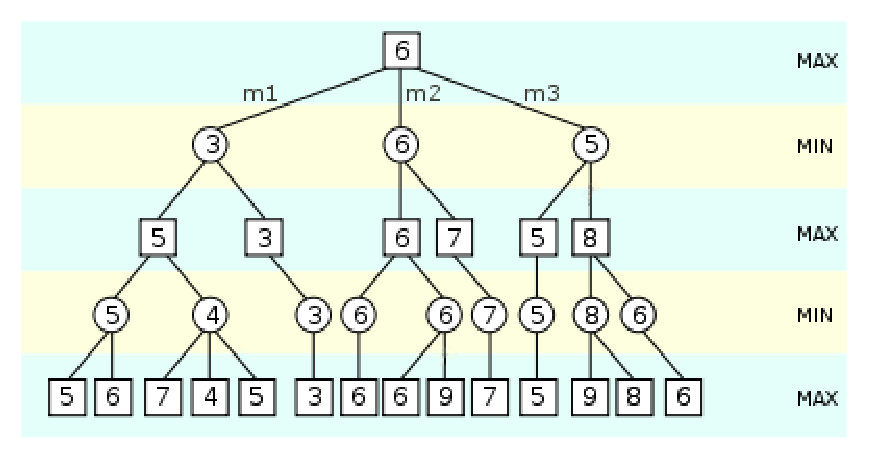
\includegraphics[scale=0.8]{contenido/cap3/imagenes/minimax.eps}
	\caption{Minimax aplicado a un árbol de juegos.}
	\label{fig:minimax}
\end{figure}

Se realiza una exploración hacia delante, generando primero el árbol completo a una determinada profundidad (cuatro en este caso), a continuación se evalúan las hojas con la función de utilidad y los valores se propagan hacia arriba de la siguiente forma:
\begin{itemize}
\renewcommand{\labelitemi}{-}
	\item Un nodo \textit{MAX} toma como valor el máximo de sus hijos.
	\item Un nodo \textit{MIN} toma como valor el mínimo de sus hijos.
\end{itemize}
Finalmente, el movimiento de \textit{MAX} es el mejor valorado de sus hijos inmediatos, que en el caso de la figura~\ref{fig:minimax} se trata del movimiento \textit{m2}.

Esta forma de proceder es más fiable que evaluar solamente los hijos inmediatos, como hacía el agente evaluador heurístico presentado en la sección~\ref{ssec:evaluador_heuristico}.
La función de utilidad que usa minimax para asignar los valores a los nodos evaluados es una función de evaluación heurística, puesto que en la mayoría de los casos los estados a evaluar no serán terminales.
Esta función se define en el capítulo~\ref{cap:heuristicos} dedicado a los evaluadores heurísticos.

El algoritmo minimax realiza una exploración primero en profundidad.
Para una búsqueda en un árbol a profundidad \textit{p} y un factor de ramificación \textit{b}, minimax evaluará $b^p$ nodos hojas.
La complejidad en tiempo del algoritmo minimax es $O(b^p)$; y la complejidad en espacio es $O(bp)$ si se generan todos los sucesores a la vez, o $O(p)$ si se generan uno por uno.
Para juegos reales, los costes de tiempo son impracticables, pero este algoritmo sirve como base para el análisis matemático de juegos y para otros algoritmos más prácticos.

Existen numerosas mejoras del algoritmo minimax original; algunas de ellas consisten en realizar:
\begin{itemize}
	\item una búsqueda en profundidad con retroceso (\textit{backtrack}),
	\item una búsqueda con profundización progresiva (\textit{algoritmos anytime}),
	\item explorar sólo la parte imprescindible del árbol (\textit{poda alfa-beta}), o
	\item almacenar información sobre los estados visitados anteriormente  y usarla cuando nos encontremos esos estados por otro camino del árbol (\textit{tablas de transposiciones}).
\end{itemize}
A continuación se detallan cada una de estas mejoras que se han implementado e incorporado a la aplicación; presentando primero la variante implementada del algoritmo minimax: negamax.

\subsubsection{Negamax}
\label{sssec:negamax}
En lugar del algoritmo minimax propiamente dicho se ha implementado una variante equivalente conocida como \textbf{negamax}.
En esta variante, cada nodo del árbol de juegos toma siempre el valor máximo de sus hijos, independientemente de que sea un nodo \textit{MAX} o \textit{MIN}.
Adicionalmente, los valores de los nodos \textit{MAX} se cambian de signo.
De este modo, es equivalente para un nodo \textit{MIN} tomar el máximo de las evaluaciones cambiadas de signo, que tomar el mínimo de las evaluaciones sin alterar.
El origen de negamax se basa en la igualdad matemática:
\begin{displaymath}
\max{(x, y)} = - \min{(-x, -y)}
\end{displaymath}

Negamax no supone una mejora directa de minimax, sino que se trata más bien del algoritmo minimax comprimido que evita tener que definir dos funciones distintas para \textit{MAX} y \textit{MIN}.
Además, se sigue teniendo el mismo problema de la complejidad que supone explorar el árbol de juegos al completo.
Para evitar esto se ha modificado la versión original de negamax dando lugar a dos agentes que emplean dos estrategias diferentes: una con profundidad máxima de búsqueda y otra con un límite de tiempo.

\subsubsection{Minimax con profundidad máxima de búsqueda}
\label{sssec:profundidad_maxima_busqueda}
El primer agente emplea una estrategia con la variante negamax y un parámetro adicional que indica la profundidad máxima de búsqueda en el árbol de juegos a partir de la posición actual.

La estrategia comienza en la posición actual y realiza una búsqueda en profundidad con retroceso (\textit{backtrack}) hasta la profundidad de búsqueda indicada.
Los sucesores son generados aleatoriamente de uno en uno y en cada paso el algoritmo se queda con el mejor movimiento en función del valor minimax devuelto.

% PONER ESTO EN DISEÑO.
%El algoritmo minimax y su variante negamax es recursivo por naturaleza y así ha sido implementado; aunque esto pueda parecer un inconveniente en cuanto a la eficiencia, el algoritmo resultante es muy fácil de entender y esto era uno de los objetivos de este proyecto, por encima de la eficiencia obtenida en los algoritmos.
%Además, una versión iterativa de los mismos no siempre supone una mejora en la eficiencia, debido al gran aumento en complejidad que supone desarrollar y gestionar una estructura temporal (por ejemplo una pila) para almacenar la información de la recursividad.

Este agente puede evaluar posiciones a una profundidad dada.
Sin embargo, incrementos lineales de profundidad pueden originar búsquedas que requieran un tiempo exponencialmente mayor.
Del mismo modo, aún sin variar la profundidad, el tiempo necesario para la búsqueda puede ser muy variable.
Normalmente el número de posibilidades al comienzo de un juego es mucho mayor que a medida que se desarrolla la partida, por lo que examinar los movimientos iniciales puede llevar un tiempo mayor.

La limitación del tiempo de cómputo puede superarse empleando un algoritmo que en cualquier momento pueda dar una solución, pero que proporcione soluciones mejores cuanto mayor sea el tiempo disponible.
Los algoritmos que presentan esta propiedad se conocen como algoritmos \textit{anytime}.
El siguiente agente, que también emplea una estrategia minimax, dispone de un límite de tiempo para realizar la búsqueda, en lugar de un límite en la profundidad máxima de búsqueda.

\subsubsection{Minimax con límite de tiempo}
\label{sssec:limite_tiempo}
El segundo agente también emplea negamax pero dispone de un tiempo limitado para realizar la búsqueda del mejor movimiento en el árbol de juegos.

Se trata de un algoritmo \textit{anytime}.
Un \textbf{algoritmo \textit{anytime}} devuelve una solución cuya calidad depende del tiempo de cómputo disponible.
El algoritmo encontrará mejores soluciones a medida que aumenta el tiempo disponible para realizar la búsqueda.

La estrategia realiza una búsqueda con retroceso y profundización progresiva (\textit{Backtrack with Iterative Deepening}.
La búsqueda dispone de una cota (profundidad máxima de búsqueda) que se incrementa automáticamente en cada iteración.
El algoritmo guarda siempre la mejor jugada inmediata para la última exploración realizada con objeto de devolverla cuando el tiempo se acabe.
En cada iteración el algoritmo comprueba el tiempo restante, terminando la búsqueda cuando este se agota.

Puede darse el caso de que el límite de tiempo sea tan pequeño que la estrategia no tenga tiempo de devolver un movimiento, en ese caso el agente acabará realizando un movimiento aleatorio.
Además, para asegurarse de devolver el mejor movimiento, la estrategia debe evaluar todos los nodos del nivel del árbol que corresponde a la cota de la iteración actual.
Si en la iteración actual no ha tenido tiempo de evaluarlos todos, devolverá el mejor movimiento obtenido en la iteración anterior.

Por simplicidad, la unidad de tiempo escogida ha sido el segundo, pues para la mayoría de juegos no tiene sentido dejar menos tiempo de cómputo al agente debido a la complejidad de los propios juegos.
Esto implica que el tiempo mínimo permitido sea de un segundo.
